% "Incorrect figure numbering when using subfloats in a subfloatrow"
% http://tex.stackexchange.com/questions/52029/subfloats-in-a-subfloatrow-seem-to-be-making-figures-be-numbered-wrong-how-can

% I have a document with a lot of subfigures which are different heights and need to be placed side-by-side and centered vertically. It seems like the floatrow package is ideal for this.
%
% After much trial and error, I finally made it through the documentation enough to get the subfloats to center correctly, but now every time there is a subfloat, the figure counter gets incremented, so I have figure 10 followed by figure 13, when figure 10 has two subfloats in it. In the minimal example, notice that the single figure in the document is labelled Figure 3!
%
% There was a similar question floating around the web about 5 years ago, but I didn't see an answer.
%
% Here's minimal code:

\iffalse
\documentclass[11pt]{article}
\usepackage{subfig}  
\usepackage{tikz}

\usepackage[]{floatrow} 
\floatsetup[figure]{floatrowsep=qquad,valign=c }
\floatsetup[subfloat]{subfloatrowsep=qquad,valign=c}
\usepackage{graphicx}

\begin{document}

\begin{figure}[htbp]
\centering
\ffigbox{
\begin{subfloatrow}[3]
\subfloat[First, we see an empty green circle]{
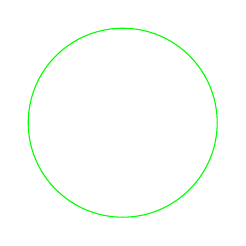
\begin{tikzpicture}[scale=1] \draw[green]  (0,0) circle (1.2cm);\end{tikzpicture}
}

\subfloat[A large orange circle is the middle picture]{
\begin{tikzpicture}[scale=1]\draw[orange] (0,0) circle (2cm);\end{tikzpicture}}

\subfloat[Finally, a beautiful red circle with a black border]{

\begin{tikzpicture}[scale=1]\draw[fill=red]  (0,0) circle (.75cm);\end{tikzpicture}}
\end{subfloatrow}
}
{\caption{``Gadgets'' in reduced Levi graphs found as a consequence of using the construction in the configuration construction lemma.}
\label{CCLvolt}
}
\end{figure}
\end{document}
\fi

\documentclass[11pt]{article}
\usepackage{subcaption}  
\usepackage{tikz}

\usepackage[]{floatrow} 
\floatsetup[figure]{floatrowsep=qquad,valign=c }
\floatsetup[subfloat]{subfloatrowsep=qquad,valign=c}
\usepackage{graphicx}

\begin{document}

\begin{figure}[htbp]
\centering
\ffigbox{
\begin{subfloatrow}[3]
\subcaptionbox{First, we see an empty green circle}{
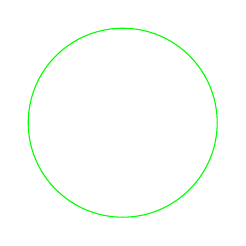
\begin{tikzpicture}[scale=1] \draw[green]  (0,0) circle (1.2cm);\end{tikzpicture}
}

\subcaptionbox{A large orange circle is the middle picture}{
\begin{tikzpicture}[scale=1]\draw[orange] (0,0) circle (2cm);\end{tikzpicture}}

\subcaptionbox{Finally, a beautiful red circle with a black border}{

\begin{tikzpicture}[scale=1]\draw[fill=red]  (0,0) circle (.75cm);\end{tikzpicture}}
\end{subfloatrow}
}
{\caption{``Gadgets'' in reduced Levi graphs found as a consequence of using the construction in the configuration construction lemma.}
\label{CCLvolt}
}
\end{figure}
\end{document}

